% !TeX root = ../main-paper.tex
\section{Results}

\subsection{Experiment 1: NER sensibility to the number of training samples}

Qualitative results
\textbf{TODO random samples of results + selection of failure cases}


Quantitative results: table + graph ideally (with training set size info)

\begin{table}[!h]

\caption{Models F1 score on unseen data vs trainset size}
\centering
\begin{tabular}[t]{lcccccccc}
\toprule
Trainset size (entries) & 49 & 99 & 199 & 398 & 796 & 1593 & 3186 & 6373\\
Trainset size (\% of the full trainset) & 0.8 & 1.5 & 3.1 & 6.2 & 12.5 & 25 & 50 & 100\\
\midrule
Cnn & \textbf{0.855} & \textbf{0.885} & \textbf{0.910} & 0.911 & 0.919 & 0.925 & 0.926 & 0.929\\
Camembert & 0.236 & 0.626 & 0.856 & \textbf{0.916} & \textbf{0.930} & 0.933 & \textbf{0.948} & 0.953\\
Camembert+pretraining & 0.190 & 0.685 & 0.889 & 0.913 & \textbf{0.930} & \textbf{0.946} & \textbf{0.948} & \textbf{0.960}\\
\bottomrule
\end{tabular}
\end{table}

\begin{figure}[htb!]
	   \center{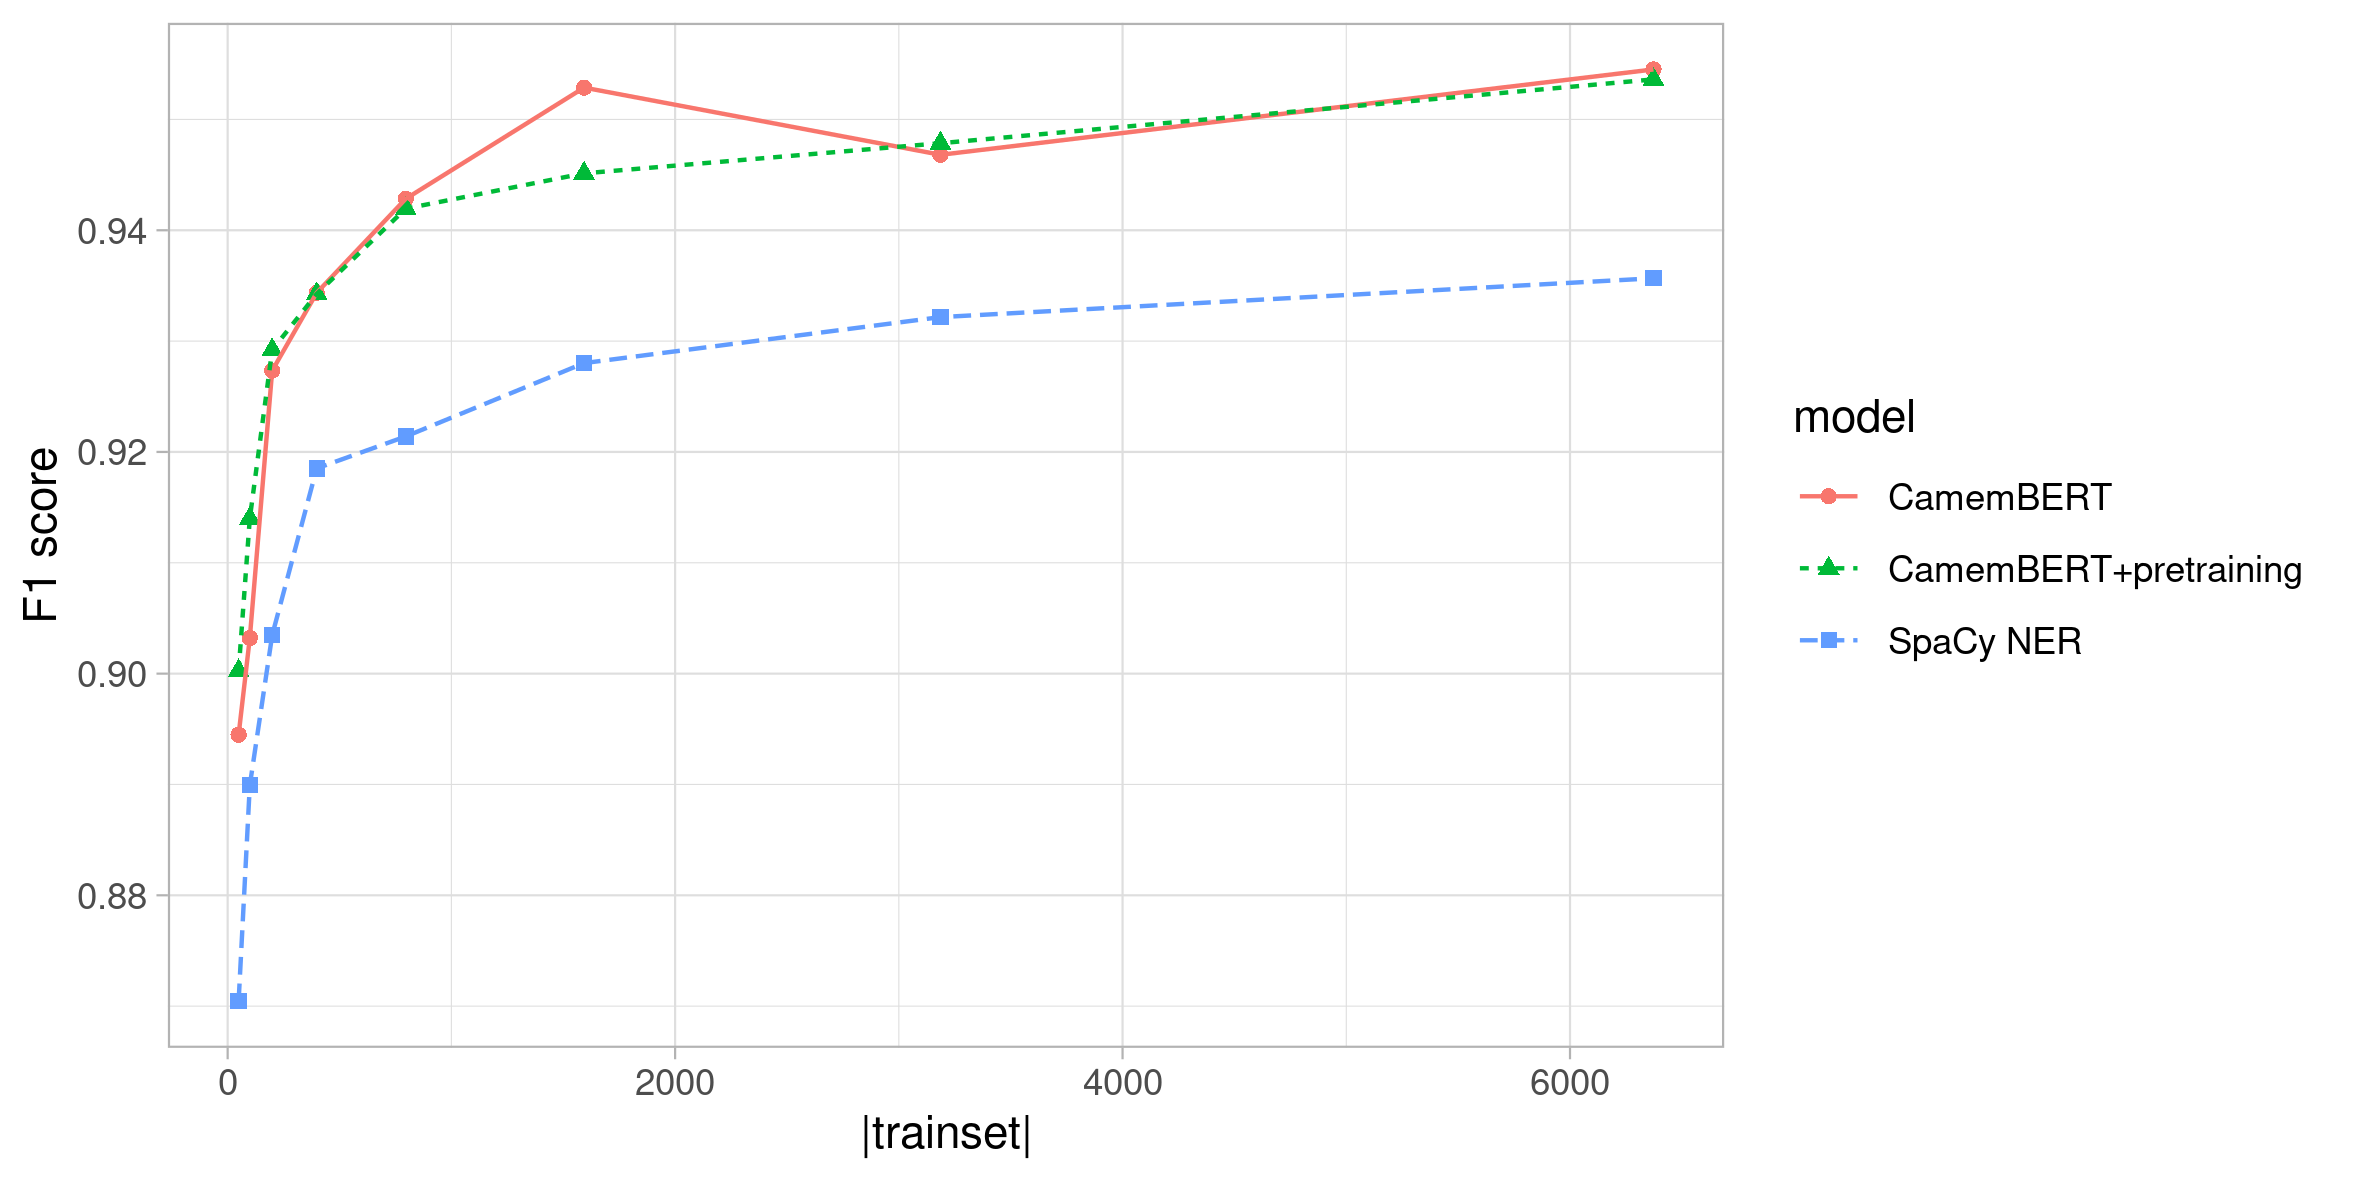
\includegraphics[width=\textwidth]
	       {../material/experiment_1/f1_vs_trainsize.png}}
	  \vspace{3in}
	  \caption{\label{fig:f1-vs-trainsize} Models F1 score on unseen data vs trainset size}
\end{figure}
	                                        


\subsection{Experiment 2: NER in the presence of noisy OCR texts}

Qualitative results
\textbf{TODO random samples of results + selection of failure cases}

Quantitative results: table + graph ideally (with OCR noise, same format as previous)

Table : NER NN models VS train on {noisy, clean} datasets VS evaluate on {noisy, clean} datasets


\begin{table}[h!]
\caption{Camembert vs noise}
\centering
\begin{tabular}{ll|cc|c}
 & & \multicolumn{2}{c|}{Training data} & \\
 & & noisy & clean &   \\ 
\cline{1-4}
\multirow{3}{*}{Test data}& noisy gold (Tesseract) & f1 & f1 & \\
                            & noisy gold (Pero-OCR) & f1 & f1 & \\ 
                            & reference gold & f1 & f1 & \\ 
\cline{1-4}
                            & \multicolumn{1}{l}{} &       & \multicolumn{1}{l}{}       &   \\
                            & \multicolumn{1}{l}{} &       & \multicolumn{1}{l}{}       &  
\end{tabular}
\end{table}



Opt. use synthetic text perturbation as well? Maybe not interesting and too artificial if we have access to 2+ OCR systems.
(original OCR from BNF, Tesseract 4, Pero OCR…)


\subsection{Discussion}
Interesting points to discuss:
\begin{itemize}
    \item can we train on noisy data? (without manual OCR correction?) => future work? cf Pero OCR training procedure?
    \item do we need better OCR systems or better post-correction techniques (if NER is reliable enough)?
    \item Construction of the lexicon and associated cost
\end{itemize}
